% !TEX program = latexmk

\documentclass{article}
\usepackage{paper0}
\usepackage{setspace}
\usepackage{geometry}
\usepackage{enumitem}
\usepackage{ctex}
\usepackage{xeCJK}
\usepackage{amsmath}
\usepackage{fontspec}
% \usepackage{mathspec}
% \usepackage[bold-style=ISO]{unicode-math}
% \usepackage{mathptmx}
\usepackage{txfonts}
\usepackage[T1]{fontenc}
\usepackage{fancyhdr}
\usepackage{lastpage}
\usepackage{esvect}
\usepackage{graphicx}
\usepackage{caption}
\usepackage{cases}
\usepackage{wrapfig}

\geometry{
    paper = a4paper,
    top = 3cm,  % 上边距
    bottom = 3cm,  %下边距
    left= 2.5cm,   %左边距
    right = 2.5cm   %右边距
}

% \setcounter{tocdepth}{2}
\setstretch{1.3}
\setCJKmainfont{STZHONGS.TTF}[Path=fonts/]
\setmainfont{Times New Roman}
\pagestyle{fancy}
\renewcommand{\headrulewidth}{0pt}

\begin{document}

\lfoot{}
\rfoot{}
\cfoot{}
\firstpage{2024}{数学}

\newpage

\lfoot{上海市教育考试院~~{\heiti 保留版权}}
\rfoot{2024年上海市初中学业水平考试~~数学试卷~~第1页(共4页)}
\cfoot{}

\ptitle{2024}{数学}

\setstretch{1.5}

\qtitle{一、选择题:(本大题共6题,每题4分,满分24分.每题只有一个选项是正确的)}

\begin{question}[1]
    \item 如果$x>y$,那么下列正确的是
    \onp{$x+5<y+5$}{$x-5<y-5$}{$5x>5y$}{$-5x>-5y$}
\end{question}

\begin{question}[2]
    \item 如果$f(x)=\dfrac{2-x}{x-3}$,那么下列正确的是
    \onp{$x=2$}{$x\neq 2$}{$x=3$}{$x\neq 3$}
\end{question}

\begin{question}[3]
    \item 以下一元二次方程有两个相等实数根的是
    \onp{$x^2-6x=0$}{$x^2-9=0$}{$x^2-6x+6=0$}{$x^2-6x+9=0$}
\end{question}

\begin{question}[4]
    \item 科学家同时培育了甲乙丙丁四种花,这四种花开花时间最短且最平稳的是
    \begin{center}
        \begin{tabular}{|c|c|c|c|c|} \hline
            种类 & 甲种类 & 乙种类 & 丙种类 & 丁种类 \\ \hline
            平均数 & 2.3 & 2.3 & 2.8 & 3.1 \\ \hline
            方差 & 1.05 & 0.78 & 1.05 & 0.78 \\ \hline
        \end{tabular}
    \end{center} \leavevmode
    \onps{甲种类}{乙种类}{丙种类}{丁种类}
\end{question}

\begin{question}[5]
    \item 四边形$ABCD$为矩形,过$A$、$C$作对角线$BD$的垂线,过$B$、$D$作对角线$AC$的垂线.如果这四条垂线可以组成一个四边形,那这个四边形为
    \onp{菱形}{矩形}{直角梯形}{等腰梯形}
\end{question}

\begin{question}[6]
    \item 在$\triangle ABC$中,$AC=3$,$BC=4$,$AB=5$,点$P$在$\triangle ABC$内,分别以$A$、$B$、$P$为圆心画圆,
          $r_A=1$,$r_B=2$,$r_P=3$,$\odot A$与$\odot P$内切,则$\odot P$与$\odot B$的关系是
    \onp{内含}{外切}{相交}{相离}
\end{question}

\qtitle{二、填空题:(本大题共12题,每题4分,满分48分)}

\begin{question}[7]
    \item 计算:$(4x^2)^3=$\blank .
\end{question}

\begin{question}[8]
    \item 计算:$(a+b)(b-a)=$\blank .
\end{question}

\begin{question}[9]
    \item 已知$\sqrt{2x-1}=1$,则$x=$\blank .
\end{question}

\newpage

\lfoot{2024年上海市初中学业水平考试~~数学试卷~~第2页(共4页)}
\rfoot{}
\cfoot{}

\begin{question}[10]
    \item 科学家研发了一种新的蓝光唱片,一张蓝光唱片的容量约为$2\times 10^5$GB,一张普通唱片的容量约为25GB,
          则蓝光唱片的容量是普通唱片的\blank 倍.
\end{question}

\begin{question}[11]
    \item 如果正比例函数$y=kx$的图像经过点$(7,-13)$,则$y$的值随$x$的增大而\blank (选填“增大”或“减小”).
\end{question}

\begin{question}[12]
    \item 在菱形$ABCD$中,$\angle ABC=66^\circ$,则$\angle BAC=$\blank $^\circ$.
\end{question}

\begin{question}[13]
    \item 某种商品的销售量$y$(万元)与广告投入$x$(万元)成一次函数关系,当投入10万元时销售额1000万元,
          当投入90万元时销售额5000万元,则投入80万元时,销售额为\blank 元.
\end{question}

\begin{question}[14]
    \item 一个袋子中有若干个白球和绿球,它们除了颜色外都相同.随机从中摸一个球,恰好摸到绿球 \\[5pt]
          的概率是$\dfrac{3}{5}$,则袋子中至少有\blank 个绿球.
\end{question}

\begin{question}[15]
    \item 如图1,在平行四边形$ABCD$中,$E$为对角线$AC$上一点,设$\vv{AC}=\vv{a}$,
          $\vv{BE}=\vv{b}$,若$AE=2EC$,则$\vv{DC}=$\blank
          (结果用含$\vv{a}$,$\vv{b}$的式子表示).
\end{question}

\begin{figure}[htbp]
    \centering
    \begin{minipage}[b]{.4\linewidth}
        \centering
        \begin{center}
            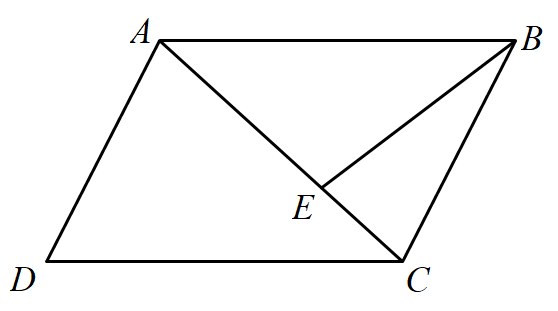
\includegraphics[scale=0.3]{images/p1.png}
            \caption*{图1}
        \end{center}
    \end{minipage}
    \qquad
    \begin{minipage}[b]{.4\linewidth}
        \centering
        \begin{center}
            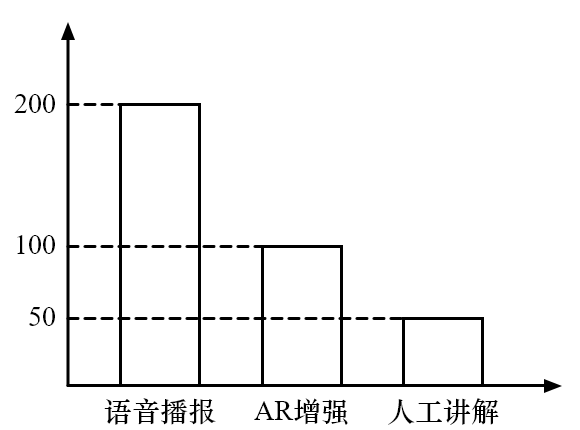
\includegraphics[scale=0.3]{images/p2.png}
            \caption*{图2}
        \end{center}
    \end{minipage}
\end{figure}

\begin{question}[16]
    \item 博物馆为展品准备了人工讲解、语音播报和AR增强三种讲解方式,为了解游客偏好,共下发并回收有效问卷1000张,
          其中700人没有讲解需求,剩余300人中需求情况如图2所示(一人可以选择多种).
          那么在总共2万人的参观中,需要AR增强讲解的人数约有\blank 人.
\end{question}

\begin{question}[17]
    \item 在平行四边形$ABCD$中,$\angle ABC$是锐角,将$CD$沿着直线$l$翻折至$AB$所在直线,对应点分别为$C'$、$D'$,
          若$AC':AB:BC=1:3:7$,则$\cos \angle ABC=$\blank .
\end{question}

\begin{question}[18]
    \item 对于一个二次函数$y=a(x-m)^2+k~(a\neq 0)$中存在一点$P(x',y')$,使得$x'-m=y'-k\neq 0$,则称 \\[5pt]
          $2|x'-m|$为该抛物线的“开口大小”,那么抛物线$y=-\dfrac{1}{2}x^2+\dfrac{1}{3}x+3$的“开口大小”为\blank .
\end{question}

\qtitle{三、解答题:(本大题共7题,满分78分)}

\begin{question}[19]
    \item (本题满分10分)\\[5pt]
          计算:$|1-\sqrt{3}|+24^\frac{1}{2}+\dfrac{1}{2+\sqrt{3}}-(1-\sqrt{3})^0$.
\end{question}

\newpage

\lfoot{}
\rfoot{2024年上海市初中学业水平考试~~数学试卷~~第3页(共4页)}
\cfoot{}

\begin{question}[20]
    \item (本题满分10分)\\[5pt]
        解方程组:
        $\left\{
            \begin{array}{lr}
            x^2-3xy-4y^2=0 & \text{\normalsize{\textcircled{\small{1}}}\normalsize\enspace} \\
            x+2y=6 & \text{\normalsize{\textcircled{\small{2}}}\normalsize\enspace}
        \end{array}\right.$.
\end{question} \leavevmode \\

\begin{question}[21]
    \item (本题满分10分,第(1)题4分,第(2)题6分)\\[5pt]
    \begin{minipage}[t]{.6\textwidth}
        如图3,在平面直角坐标系$xOy$中,反比例函数$y=\dfrac{k}{x}$($k$为 \\[5pt]
        常数且$k\neq 0$)上有一点$A(-3,m)$,且与直线$y=-2x+4$交于另一点$B(n,6)$.
        \begin{squestion}
            \item 求$k$与$m$的值;
            \item 过点$A$作直线$l~//~x$轴与直线$y=-2x+4$交于点$C$,求$\sin \angle OCA$的值.
        \end{squestion}
    \end{minipage}
    \begin{minipage}[t]{.4\textwidth}
        \centering
        \vspace{-2ex}
        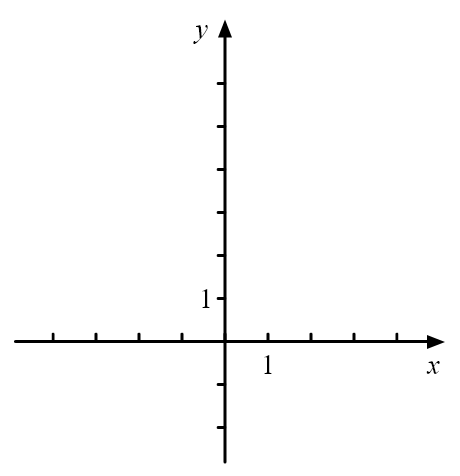
\includegraphics[scale=0.3]{images/p3.png}
        \captionof*{figure}{图3}
    \end{minipage}
\end{question} \leavevmode

\begin{question}[22]
    \item (本题满分10分,第(1)题6分,第(2)题4分)\\
    \begin{minipage}[t]{.6\textwidth}
        数学小组用两副相同的三角板(分别是含$45^\circ$的直角三角板和含$60^\circ$的直角三角板)
        拼出如图4所示的平行四边形,已知任意一副三角板的两个直角三角形斜边上的高都为$h$.
        \begin{squestion}
            \item \begin{ssquestion}
                \item 用$h$表示两种三角形的直角边;
                \item 用$h$表示中间阴影部分的面积.
            \end{ssquestion}
            \item 用这两副三角板拼出不同于右图所示的平行四边形(不需要标出角度,作出三角形的边即可).
        \end{squestion}
    \end{minipage}
    \begin{minipage}[t]{.4\textwidth}
        \centering
        \vspace{-2ex}
        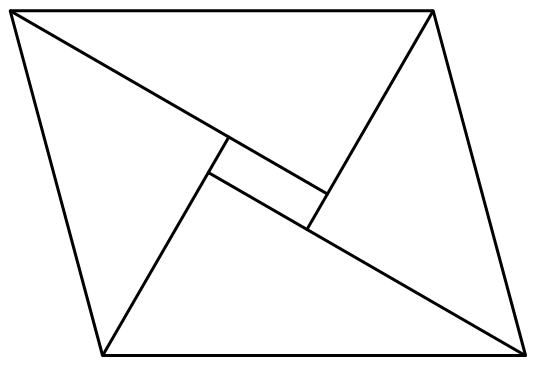
\includegraphics[scale=0.25]{images/p4.png}
        \captionof*{figure}{图4}
    \end{minipage}
\end{question} \leavevmode \\

\begin{question}[23]
    \item (本题满分12分,第(1)题5分,第(2)题7分)\\
    \begin{minipage}[t]{.58\textwidth}
        如图5,在矩形$ABCD$中,$E$为边$CD$上一点,且$AE\perp BD$.
        \begin{squestion}
            \item 求证:$AD^2=DE\cdot DC$;
            \item \vspace{0.1cm} 设$F$为线段$AE$延长线上一点,且$EF=CF=\dfrac{1}{2}BD$,\\[5pt]
                  求证:$CE=AD$.
        \end{squestion}
    \end{minipage}
    \begin{minipage}[t]{.42\textwidth}
        \centering
        \vspace{-2ex}
        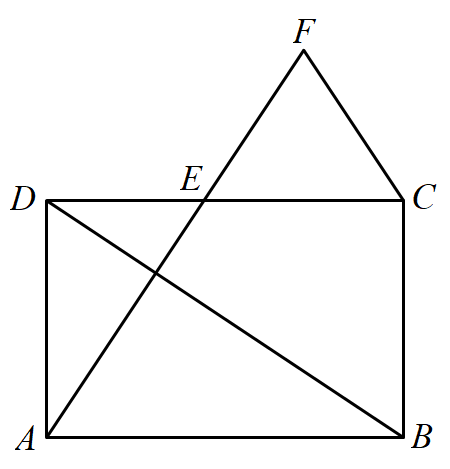
\includegraphics[scale=0.3]{images/p5.png}
        \captionof*{figure}{图5}
    \end{minipage}
\end{question} \leavevmode

\newpage

\lfoot{2024年上海市初中学业水平考试~~数学试卷~~第4页(共4页)}
\rfoot{}
\cfoot{}

\begin{question}[24]
    \item (本题满分12分,第(1)题4分,第(2)题8分)\\[5pt]
    在平面直角坐标系$xOy$中,抛物线$y=\dfrac{1}{3}x^2$平移后的图像经过点$A(0,-\dfrac{5}{3})$和$B(5,0)$.\\[5pt]
    \begin{minipage}[t]{.6\textwidth}
        \begin{squestion}
            \item 求平移后新抛物线的表达式;
            \item 直线$x=m~(m>0)$与新抛物线交于点$P$,与原抛物线交于点$Q$.
            \begin{ssquestion}
                \item 当$PQ<3$时,求$m$的取值范围;
                \item 记点$P$在原抛物线上的对应点为$P'$,如果四边形$P'BPQ$有一组对边平行,求点$P$的坐标.
            \end{ssquestion}
        \end{squestion}
    \end{minipage}
    \begin{minipage}[t]{.4\textwidth}
        \centering
        \vspace{-2ex}
        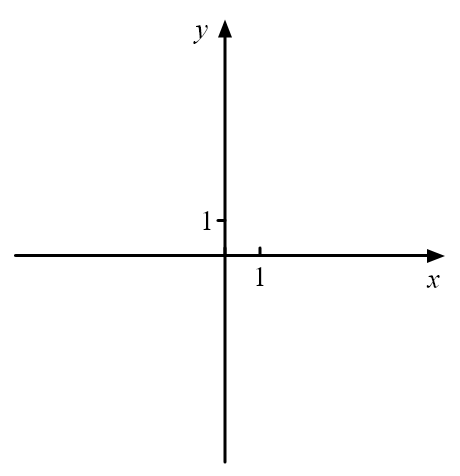
\includegraphics[scale=0.3]{images/p6.png}
        \captionof*{figure}{图6}
    \end{minipage}
\end{question} \leavevmode \\[20pt]

\begin{question}[25]
    \item (本题满分14分,第(1)题4分,第(2)题10分)\\[5pt]
    在梯形$ABCD$中,$AD~//~BC$,点$E$在边$AB$上,且$AE=\dfrac{1}{3}AB$.
    \begin{squestion}
        \item \vspace{0.1cm} 如图7所示,点$F$在边$CD$上,且$DF=\dfrac{1}{3}DC$,联结$EF$,求证:$EF~//~BC$;
        \item \vspace{0.1cm} 当$AD=AE=1$时:
        \begin{ssquestion}
            \item 如图8,联结$DE$,如果$\triangle ADE$的外接圆的圆心恰好落在$\angle B$的角平分线上,
                  求$\triangle ADE$的外接圆的半径长;
            \item \vspace{0.1cm} 如图9,如果点$M$在边$BC$上,联结$EM$、$DM$、$EC$,$DM$与$EC$交于$N$.
                  如果$BC=4$,$CD^2=DN\cdot DM$且$\angle DMC=\angle CEM$,求边$CD$的长.
        \end{ssquestion}
    \end{squestion}
\end{question} \leavevmode \\

\noindent\begin{minipage}[b]{.24\textwidth}
    \centering
    \vspace{-2ex}
    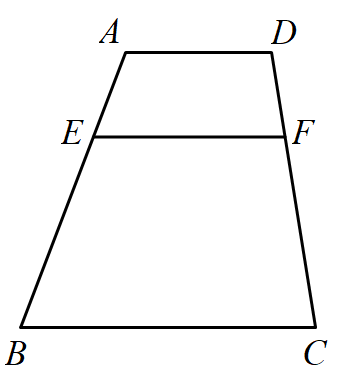
\includegraphics[scale=0.3]{images/p7.png}
    \captionof*{figure}{图7}
\end{minipage}
\begin{minipage}[b]{.36\textwidth}
    \centering
    \vspace{-2ex}
    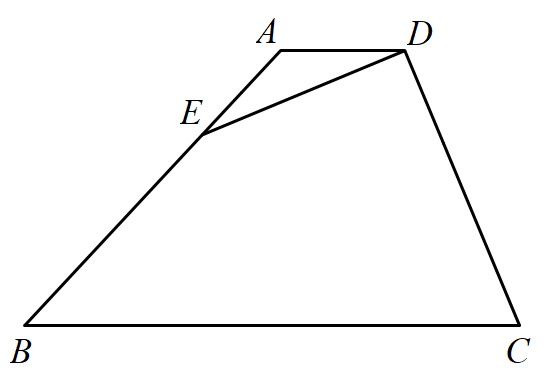
\includegraphics[scale=0.3]{images/p8-2.png}
    \captionof*{figure}{图8}
\end{minipage}
\begin{minipage}[b]{.44\textwidth}
    \centering
    \vspace{-2ex}
    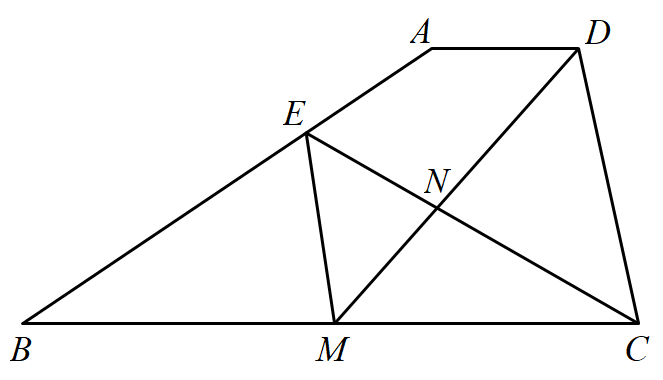
\includegraphics[scale=0.3]{images/p9-2.png}
    \captionof*{figure}{图9}
\end{minipage}

\end{document}